\documentclass{exam}
\usepackage[utf8]{inputenc}
\usepackage{lmodern}
\usepackage{microtype}

% \usepackage[parfill]{parskip}
\usepackage[dvipsnames]{xcolor}
\usepackage{amsmath}
\usepackage{amsfonts}
\usepackage{amsthm}
\usepackage{siunitx}
\DeclareSIUnit\year{yr}
\DeclareSIUnit\foot{ft}
\DeclareSIUnit\litre{\liter}

\usepackage{skull}

\usepackage{pgfplots}
\usepgfplotslibrary{polar}
\pgfplotsset{compat=1.11}
\usepgfplotslibrary{statistics}
\usepackage{graphicx}
\usepackage{sidecap}
\sidecaptionvpos{figure}{c}
\usepackage{float}
\usepackage{gensymb}
\usepackage{tkz-euclide}
\usetkzobj{all}
\usepackage{commath}
\usepackage{hyperref}
\usepackage{enumitem}
\usepackage{wasysym}
\usepackage{multicol}
\usepackage{mathtools}
\usepackage{tcolorbox}
\usepackage{tabularx}
\usepackage[version=4]{mhchem}
\usepackage{changepage}
\usepackage{listings}
\lstset{basicstyle=\ttfamily\linespread{0.8}\small}

\renewcommand*{\thefootnote}{\fnsymbol{footnote}}

\newtheorem*{thm}{Theorem}
\newtheorem*{iden}{Identity}
\newtheorem*{lemma}{Lemma}
\newtheorem{obs}{Observation}
\theoremstyle{definition}
\newtheorem*{defn}{Definition}
\newtheorem*{ex}{Example}
\newtheorem{con}{Construction}
\newtheorem*{alg}{Algorithm}

\newtheoremstyle{break}
  {\topsep}{\topsep}%
  {\itshape}{}%
  {\bfseries}{}%
  {\newline}{}%
\theoremstyle{break}
\newtheorem*{bthm}{Theorem}

% russian integral
\usepackage{scalerel}
\DeclareMathOperator*{\rint}{\scalerel*{\rotatebox{17}{$\!\int\!$}}{\int}}

% \DeclareMathOperator*{\rint}{\int}

\pgfplotsset{vasymptote/.style={
    before end axis/.append code={
        \draw[densely dashed] ({rel axis cs:0,0} -| {axis cs:#1,0})
        -- ({rel axis cs:0,1} -| {axis cs:#1,0});
    }
}}

% \pointsinrightmargin
\boxedpoints
\pointname{}

\newcommand{\questioA}{\question[\texttt{\textbf{\color{Cerulean} A}}]}
\newcommand{\questioM}{\question[\texttt{\textbf{\color{PineGreen} M}}]}
\newcommand{\questioE}{\question[\texttt{\textbf{\color{WildStrawberry} E}}]}
\newcommand{\questioS}{\question[\texttt{\textbf{\color{Goldenrod} S}}]}
\newcommand{\questioO}{\question[\texttt{\textbf{\color{BurntOrange} O}}]}

\newcommand{\parA}{\part[\texttt{\textbf{\color{Cerulean} A}}]}
\newcommand{\parM}{\part[\texttt{\textbf{\color{PineGreen} M}}]}
\newcommand{\parE}{\part[\texttt{\textbf{\color{WildStrawberry} E}}]}
\newcommand{\parS}{\part[\texttt{\textbf{\color{Goldenrod} S}}]}
\newcommand{\parO}{\part[\texttt{\textbf{\color{BurntOrange} O}}]}

\newcommand{\subparA}{\subpart[\texttt{\textbf{\color{Cerulean} A}}]}
\newcommand{\subparM}{\subpart[\texttt{\textbf{\color{PineGreen} M}}]}
\newcommand{\subparE}{\subpart[\texttt{\textbf{\color{WildStrawberry} E}}]}
\newcommand{\subparS}{\subpart[\texttt{\textbf{\color{Goldenrod} S}}]}
\newcommand{\subparO}{\subpart[\texttt{\textbf{\color{BurntOrange} O}}]}

\newcommand{\mainHeader}[2]{\section*{NCEA Level 2 Mathematics\\#1. #2}}
\newcommand{\mainHeaderHw}[2]{\section*{NCEA Level 2 Mathematics (Homework)\\#1. #2}}
\newcommand{\seealso}[1]{\begin{center}\emph{See also #1.}\end{center}}
\newcommand{\drills}[1]{\begin{center}\emph{Drill problems: #1.}\end{center}}
\newcommand{\basedon}[1]{\begin{center}\emph{Notes largely based on #1.}\end{center}}

\begin{document}

\mainHeaderIntg{17}{The Fundamental Theorem of Calculus}
Finally, we have the punchline. We state the theorems first, and then give the (optional) proofs at the end.

\subsection*{Statements of theorems}
\begin{center}\itshape
  ``You can tell it's important because it has a name.\\You can tell it's \textbf{very} important because it has a \textbf{pompous} name.''
\end{center}

\begin{bthm}[First Fundamental Theorem of Calculus (FTC1)]
  Suppose $ f $ is a continuous function, and suppose $ F $ is any antiderivative of $ f $ (so $ F' = f $). Then,
  \begin{displaymath}
    \rint^b_a f(x) \dif{x} = F(b) - F(a) = \eval{F(x)}_a^b.
  \end{displaymath}
\end{bthm}

In other words, the definite integral of a function can be found by evaluating the indefinite integrals at
the endpoints. This actually follows from a much more intuitive result:

\begin{bthm}[Second Fundamental Theorem of Calculus (FTC2)]
  Suppose $ f $ is a continuous function. Then,
  \begin{displaymath}
    \od{}{x} \rint^x_a f(t) \dif{t} = f(x).
  \end{displaymath}
\end{bthm}

For some intuition, we can consider the following graph of $ y = f(x) $. The shaded area is the value of $ A(x) = \rint^x_a f(t) \dif{t} $;
then we use the fact that the area of the darker shaded area is approximated by $ h f(x) $ (base times height) to see that
\begin{displaymath}
  \frac{A(x + h) - A(x)}{h} \approx \frac{h f(x)}{h} = f(x).
\end{displaymath}
If we take limits, as we do in the proof of this theorem (given below), then this approximation becomes exact: the rate of change of
the area under a curve is simply the height of the curve.

\begin{center}
  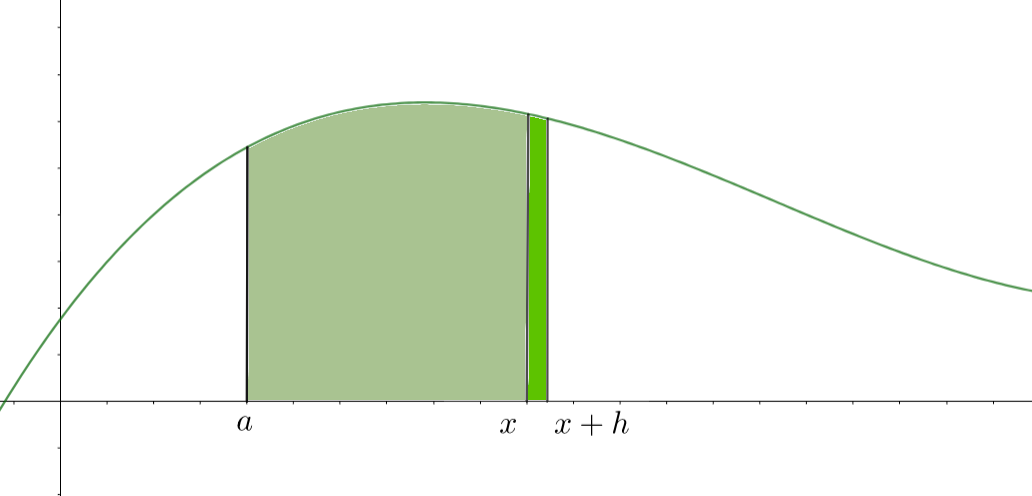
\includegraphics[width=0.6\textwidth]{ftc1}
\end{center}

\begin{joke}
  A mathematics professor was lecturing to a class of students. As he wrote something on the board,
  he said to the class ``Of course, this is immediately obvious.'' Upon seeing the blank stares of
  the students, he turned back to contemplate what he had just written. He began to pace back and
  forth, deep in thought. After about 10 minutes, just as the silence was beginning to become uncomfortable,
  he brightened, turned to the class and said, ``Yes, it IS obvious.''
\end{joke}

These theorems are \emph{fundamental} because they show us that the two main operations of calculus, integration and differentiation,
are deeply related and are (in some sense) inverses of each other. To be absolutely clear, without this theorem we would have absolutely
no justification in calling anti-derivatives `integrals' --- the second theorem tells us that if we make the upper bound of our definite integral
vary then we obtain an anti-derivative for the expression underneath the integral sign, and the first theorem tells us that if we take the definite
integral of the derivative of some function then we so happen to obtain anti-derivatives back out the other side! (In fact, notice that the indefinite
integral of $ f $ is just $ \rint^x_{f^{-1}(C)} f(x) \dif{x} $, where $ C $ is just our constant of integration!)

We also have the following theorem, which allows us to combine definite integrals together. In order to get some kind of geometric intuition,
please draw a diagram or find some kind of intuitive explanation for each!
\begin{thm}
  Suppose $ f $ and $ g $ are functions and $ \lambda $ is a real constant. Then, if the relevant integrals are defined, we have:
  \begin{enumerate}
    \item $ \displaystyle\lambda \rint_a^b f(x) \dif{x} = \rint_a^b \lambda f(x) \dif{x} $.
    \item $ \displaystyle\rint_a^b f(x) \dif{x} + \rint_a^b g(x) \dif{x} = \rint_a^b f(x) + g(x) \dif{x} $.
    \item $ \displaystyle\rint_a^a f(x) \dif{x} = 0 $.
    \item $ \displaystyle\rint_a^b f(x) \dif{x} + \rint_b^c f(x) \dif{x} = \rint_a^c f(x) \dif{x} $.
  \end{enumerate}
\end{thm}

Note that the areas below a curve are assigned \textit{negative} area!

\begin{exs}\leavevmode
  \begin{enumerate}
    \item We calculate that $ \rint^1_0 \sqrt{x} \dif{x}  = \eval{\frac{2}{3}x^{3/2}}_{x = 0}^1 = \frac{2}{3} 1^{3/2} - \frac{2}{3} 0^{3/2} = \frac{2}{3}. $
    \item The definite integral $ \rint^\pi_0 \cos x \dif{x} $ is equal to 0; this is because the (negative) area under the $ x-$axis exactly
          cancels the (positive) area above the $ x-$axis. (Draw a picture.)
    \item We calculate that $ \rint^2_0 2 \dif{x} = \eval{2x}_{x = 0}^2 = 2\cdot 2 - 2 \cdot 0 = 4 $. (Thus the integral gives us the correct value if we
          try to find the area of a square!)
  \end{enumerate}
\end{exs}


\clearpage
\subsection*{Proofs}
We will only prove the FTC for `nice' functions. We actually prove the second FTC first as it is easier, and we will state the two theorems a little
more carefully.

\begin{thm}[FTC2]
  Suppose that $ f $ is a continuous function on the closed interval $ [a,b] $.\footnote{i.e. $ f $ is continuous at every $ x $ such
  that $ a \leq x \leq b $.} Then the function $ F $ defined by
  \begin{displaymath}
    F(x) = \rint^x_a f(t) \dif{t}
  \end{displaymath}
  for all $ x $ in the closed interval $ [a,b] $ is differentiable for all $ x $ such that $ a < x < b $, and
  \begin{displaymath}
    F'(x) = \od{}{x} \rint^x_a f(t) \dif{t} = f(x).
  \end{displaymath}
\end{thm}

\begin{proof}
  Let us take the derivative in a straightforward manner.
  \begin{displaymath}
    \od{}{x} \rint^x_a f(t) \dif{t} = \lim_{h \to 0} \frac{\rint^{x + h}_a f(t) \dif{t} - \rint^{x}_a f(t) \dif{t}}{h}
                                    = \lim_{h \to 0} \frac{\rint^{x + h}_x f(t) \dif{t}}{h}.
  \end{displaymath}
  Now, let $ f(M) $ be the maximum value obtained by $ f $ on the closed interval $ [x,x+h] $; let $ f(m) $ be the minimum value. Interpreting the integral as
  an area, we have
  \begin{displaymath}
    hf(m) \leq \rint^{x + h}_x f(t) \dif{t} \leq hf(M) \implies f(m) \leq \frac{1}{h} \rint^{x + h}_x f(t) \dif{t} \leq f(M).
  \end{displaymath}
  Now, as $ h \to 0 $ we must have $ f(m) \to f(x) $ and $ f(M) \to f(x) $ (because as we make the interval smaller, $ m $ and $ M $ move towards $ x $). Hence
  \begin{displaymath}
    f(x) \leq \frac{1}{h} \rint^{x + h}_x f(t) \dif{t} \leq f(x)
  \end{displaymath}
  and so $ \od{}{x} \rint^x_a f(t) \dif{t} = f(x) $.
\end{proof}

\begin{thm}[FTC1]
  Suppose $ f $ is continuous on the closed interval $ [a,b] $, and suppose $ F $ is any antiderivative of $ f $ for all $ x $ such
  that $ a < x < b $ (so $ F'(x) = f(x) $ for all such $ x $). Then,
  \begin{displaymath}
    \rint^b_a f(x) \dif{x} = F(b) - F(a) = \eval{F(x)}_a^b.
  \end{displaymath}
\end{thm}

\begin{proof}
  Consider $ \od{}{x} \rint^x_a f(t) \dif{t} = f(x) $. In particular, $ \rint^x_a f(t) \dif{t} $ is an antiderivative of $ f $ and we can antidifferentiate both
  sides, obtaining
  \begin{equation}\label{eqn:ftc1}
    \rint^x_a f(t) \dif{t} = F(x) + C \tag{*}
  \end{equation}
  (where $ C $ is some constant). Now substitute $ a $ for $ x $ in (*): we find that $ 0 = \rint^a_a f(t) \dif{t} = F(a) + C $, and in particular $ -C = F(a) $.
  Substituting $ b $ for $ x $ in (*), we find that $ \rint^b_a f(t) \dif{t} = F(b) + C = F(b) - F(a) $; and we are done.
\end{proof}

\clearpage
\subsection*{Questions}
\begin{questions}
  \questioA Compute the following definite integrals.
    \begin{parts}
      \part $ \rint_0^1 \dif{x} $
      \part $ \rint_{-1}^{1} e^x \dif{x} $
      \part $ \rint_3^4 x^2 + 3x - 1 \dif{x} $
      \part $ \rint_0^1 x^n \dif{x} $ for integer values of $ n $.
    \end{parts}
  \questioA Find the area underneath the given curves between the given bounds:
    \begin{parts}
      \part $ y = 6x^2 + 4x + 9 $ between $ x = 0 $ and $ x = 4 $
      \part $ y = \sin x $ between $ x = 0 $ and $ x = \pi $
      \part $ y = \sin x $ between $ x = -\pi $ and $ x = \pi $
      \part $ y = \cos x $ between $ x = -\pi $ and $ x = \pi $
      \part $ y = \frac{1}{x} $ between $ x = 1 $ and $ x = 2 $
    \end{parts}
  \questioA Find all the problems in the following working.
            \begin{align*}
              \rint^{-1}_1 \frac{\dif{x}}{x} = \ln \abs{-1} - \ln \abs{1} = 0
            \end{align*}
  \questioA Show that $ \rint \ln x \dif{x} = x\ln x - x + C $.
  \questioM Let $ f $ be a function such that for all $ x $, $ f(-x) = -f(x) $. Such a function is called \textit{odd}. Show that for all $ a $,
            \begin{displaymath}
              \rint^a_{-a} f(x) \dif{x} = 0.
            \end{displaymath}
            What does this mean geometrically?
  \questioM Let $ f $ be an odd function with period 2 such that $ \rint^{1}_0 f(x) \dif{x} = k $. Compute:
    \begin{parts}
      \part $ \rint^{1}_{-1} f(x) \dif{x} $
      \part $ \rint^{-1}_0 f(x) \dif{x} $
    \end{parts}
  \questioA Let $ f $ be a function such that for all $ x $, $ f(-x) = f(x) $. Such a function is called \textit{even}. Show that for all $ a $,
            \begin{displaymath}
              \rint^a_{-a} f(x) \dif{x} = 2\rint^a_0 f(x) \dif{x}.
            \end{displaymath}
            What does this mean geometrically?
  \questioM If $ \rint^1_{-2} f(x) \dif{x} = 2 $ and $ \rint^3_1 f(x) \dif{x} = -6 $, what is the value of $ \rint_{-2}^3 f(x) \dif{x} $?
  \clearpage
  \questioM Find the area between the curves $ y = x^2 + x $ and $ y = -x^2 - x $ shaded here.
            \begin{center}
              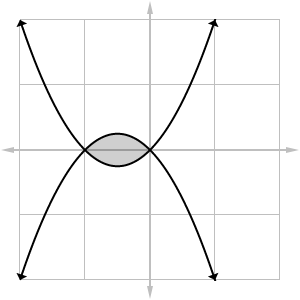
\includegraphics[width=0.3\textwidth]{int1}
            \end{center}
  \questioM Find the area between the two curves $ y = 1 + x^2 $ and $ y = 3 + x $.
  \questioM Find the area of the region bounded by $ f(x) = 4 $, $ g(x) = \frac{e^x}{5} $, and $ x = 0 $.
  \questioM What is the area of the region between the graphs of $ f(x) = 2x^2  + 5x $ and $ g(x) = -x^2 - 6x + 4 $ from $ x = -4 $ to $ x = 0 $?
  \questioE Find the area bounded by the curves $ y = \sin x $ and $ y = \cos x $ and the $ x-$axis graphed here.
            \begin{center}
              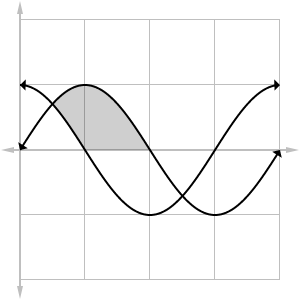
\includegraphics[width=0.2\textwidth]{int2}
            \end{center}
  \questioA Consider the function $ f $ graphed below; the total \textbf{unsigned} area between the curve and the $ x-$axis is 10 square units.
            Find $ \rint^D_A f(x) \dif{x} $.
            \begin{center}
              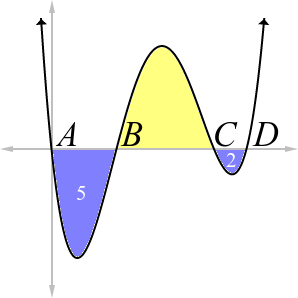
\includegraphics[width=0.3\textwidth]{int3}
            \end{center}
  \questioM
    \begin{parts}
      \part Sketch the graph of $ y = \abs{\sin x} $.
      \part Compute $ \rint^{\pi/2}_0 y \dif{x} $ using the FTC.
      \part Hence, without doing any anti-differentiation, compute $ \rint^{2\pi}_0 y \dif{x} $.
    \end{parts}
  \questioM Define $ F(x) $ by
            \begin{displaymath}
              F(x) = \rint^x_{\frac{\pi}{4}} \cos(2t) \dif{t}.
            \end{displaymath}
    \begin{parts}
      \part Use the second fundamental theorem of calculus to find $ F'(x) $.
      \part Verify part (a) by integration and differentiation.
    \end{parts}
  \questioM Compute $ \od{}{x} \rint^{x}_{2} t^t \dif{t} $.
  \questioS Scholarship 2014: Find exact expressions for the areas of the three labelled regions bounded by the two curves $ y = 9\csc^2 x $
            and $ y = 16\sin^2 x $ between $ x = \frac{\pi}{6} $ and $ x = \frac{5\pi}{6} $ shown below.
            \begin{center}
              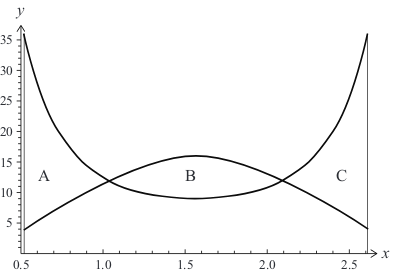
\includegraphics[width=0.5\textwidth]{schol14}
            \end{center}
\end{questions}
\end{document}
